We begin by performing a very simple screening of the available potentials using 0~K potential energy calculations.
The Fe-Al phase diagram for the relevant ideal phases in shown in Fig.~\ref{fig:0K_phases}.
Here we can already see that the potentials of Farkas \etal~\cite{farkas2020model} and Jelinek \etal~\cite{jelinek2012modified} both fail to provide clear BCC stability.
This is not shocking as these were both designed for high-entropy alloys, and the former is explicitly targeted towards the FCC phase.
Nonetheless, for the rest of our investigation we can safely focus on the EAM potential of Mendelev \etal~\cite{mendelev2005effect} and the more recent MEAM potential of Lee and Lee \etal~\cite{lee2010modified}.
%
\begin{figure}[h]
    \centering
    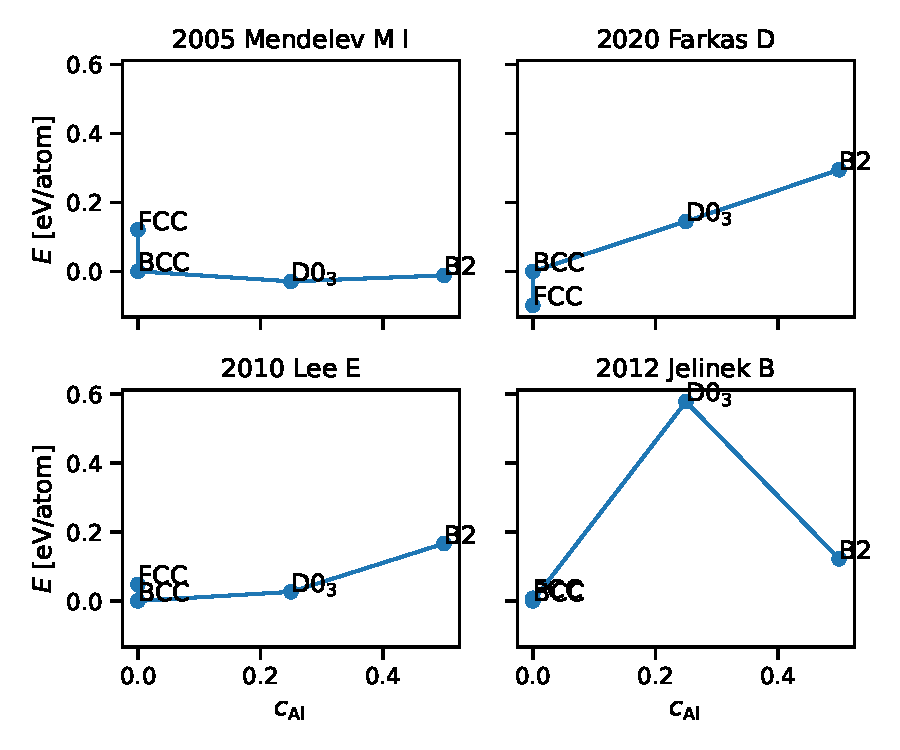
\includegraphics[width=\textwidth]{figures/zerok_phases}
    \caption{0K potential energy/atom for each of the relevant Fe-Al phases up to 50\% Al for several empirical potentials~\cite{mendelev2005effect, lee2010modified, jelinek2012modified, farkas2020model}.}
    \label{fig:0K_phases}
\end{figure}

In addition to being BCC stable, we know that the potentials should be dominated by a solid solution at 18\% Al, and that the \DOTHREE phase should also be energetically competitive such that it has the chance of appearing as small SRO clusters.
To this end, we expand the diagram in Fig.~\ref{fig:TODO} contains additional data including information about the random solid solution state at Al concentrations up to the nominal \DOTHREE concentration.
At each concentration ten different random configurations of 432 atoms ($6\times6\times6$ BCC units) we relaxed at zero pressure, and the final energy averaged over.
The error bars for the solid solution shows the 95\% confidence interval from the sampling (i.e. roughly double the standard deviation).
In addition to the solid solution and normal phases, we also show data for other ordered phases: columnar Al with varying inter-columnar spacing (similar to pin-like \BTWO precipitates) and planar Al wiht varying inter-planar spacing.
Representatives of all of these are visualized in Fig.~\ref{fig:TODO}.

In addition to the 0~K potential energy, for the solid solution data the ideal entropy of mixing was included at both the experimental annealing temperatures.
This demonstrates the increasing benefit to the \emph{free} energy for the system to occupy a disordered state.
In principle the entropy of mixing is also relevant for the other phases -- even our SRO clusters may contain chemical antisites and do not need to \emph{perfectly} conform to the reference ordering -- but at this stage they are omitted, as is vibrational entropy for all phases.
Even with these simplifications, we can already draw important conclusions: first, the Mendelev potential will never display \DOTHREE SRO at 18\% Al.
Constructing a parallel tangent line between the minima of the phases, we can expect the system is likely to form either a composition of solid solution and the layered structure, or simply form into ordered layers.
The potential energy of this layered structure sits so far below the \DOTHREE phase that we should never expect to see \DOTHREE form in any significant fraction.
Second, for the Lee potential, a similar Gibbs-tie-line analysis shows that decomposition into solid solution and \DOTHREE \emph{is} possible, but may only occur at higher temperatures than we expect from experiment.
This potential seems to have an unphysically low solubility of Al in bulk BCC Fe.

Next, to allow the full interplay and competition of all factors including vibrational entropy, we perform full MCMD calculations using the variance constrained approach~\cite{sadigh2012calculation, sadigh2012scalable} (with a relatively strict constraint $\kappa = 1e4$) to maintain the Al concentration very close to the nominal experimental value of 18\%.
Estimating the chemical potential, $\Delta \mu$ from the change in 0~K potential energies of the most favourable phases -- BCC and \DOTHREE (layered Al) for the Lee (Mendelev) potential -- gives $|\Delta \mu| < 0.1~\mathrm{eV}$ ($<0.3~\mathrm{eV}$) for the Lee (Mendelev) potential.
As seen by the inclusion of just configurational entropy to the solid solution phase, this is very likely to be an upper bound to the true chemical potential.
Since the application of the variance constraint means that the chemical potential does not ultimately influence the nature of the results obtained but only the computational efficiency (i.e. number of MC steps required) we safely approximate $\Delta \mu 0 $ for both potentials.
With a 1 fs timestep for integration, these simulations ran for 100 ps each, with MC trial swaps for 10\% of the atoms every 0.1 ps.
Although smaller than the experimental dimensions, the simulation cells were of the same order of magnitude: $4\times4\times4$ nanometer periodic cubes.
The convergence of the system to the desired chemical ordering can be seen by the good equilibration of the potential energy as a function of time in Fig.~\ref{fig:TODO}.

Unlike the experimental APT data, we have full access to the species and position of each atom in our computational sample.
Thus, to analyze SRO into the specific \DOTHREE and \BTWO configurations observed in experiment, we can directly check whether each atom has a local environment that matches the target phase.
We do this by constructing the topology of our system considering all 14 first- and second-nearest neighbours (NN) to be ``connected'', and comparing the species of the atom under question as well as all of its neighbours to one of six references: two from the \BTWO pattern with Al occupying either simple-cubic sublattice, and four symmetry-equivalent organizations of \DOTHREE.
Using a breadth-first-search, for each of the six reference patterns we construct all matching clusters.

The size and number of clusters found is then dependent on how strictly one demands that the test environment match the reference environment;
if we very strictly insist that each atom in a cluster be surrounded by \emph{exactly} the reference cluster, it is exceedingly difficult to find clusters beyond a few atoms in size given the entropic favourability of a random solution;
however, at the opposite extreme, if we are too relaxed in our condition and allow atoms with only a few neighbours matching the reference to count towards a cluster, then the entire system is consumed with one erroneous ``cluster''.
To overcome this we must make reference to the same clustering algorithm applied to the truly random solid solution used as input to the MCMD simulations, and consider the \emph{changes} in the cluster distribution after the sample has been allowed to equilibrate its chemical ordering.
In principle, one can devise a max-entropy scheme to select a threshold number of matching neighbours which optimizes the difference between the cluster distributions for the random and equilibrated samples.
In practice, we found that a threshold value of 11 of the 14 NN did a good job of this, and the interested reader can examine the \code{github} repository~\cite{feal} for more detail.

\todo{Results and plots: histograms and structures. Emphasize Bayesian prior of the initial random distribution. Highlight that we really do see planes/rods in the biggest cluster for Mendelev, and hopefully we'll see D03 for Lee!!!}